\section{Systeem}

\subsection*{Diagram}


\begin{frame}
    \frametitle{Systeemdiagram}
    
    \only<1>{
        \begin{figure}
            \centering
            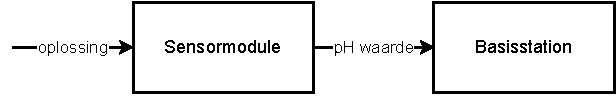
\includegraphics[width=\textwidth]{toplevelDiagram}
        \end{figure}
    }
    \only<2>{
        \begin{figure}
            \centering
            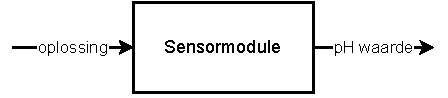
\includegraphics[width=\textwidth]{topLevelModuleOnly}
        \end{figure}
    }
\end{frame}

\transboxin


\begin{frame}
    \frametitle{Systeemdiagram}
    
    \begin{figure}
        \centering
        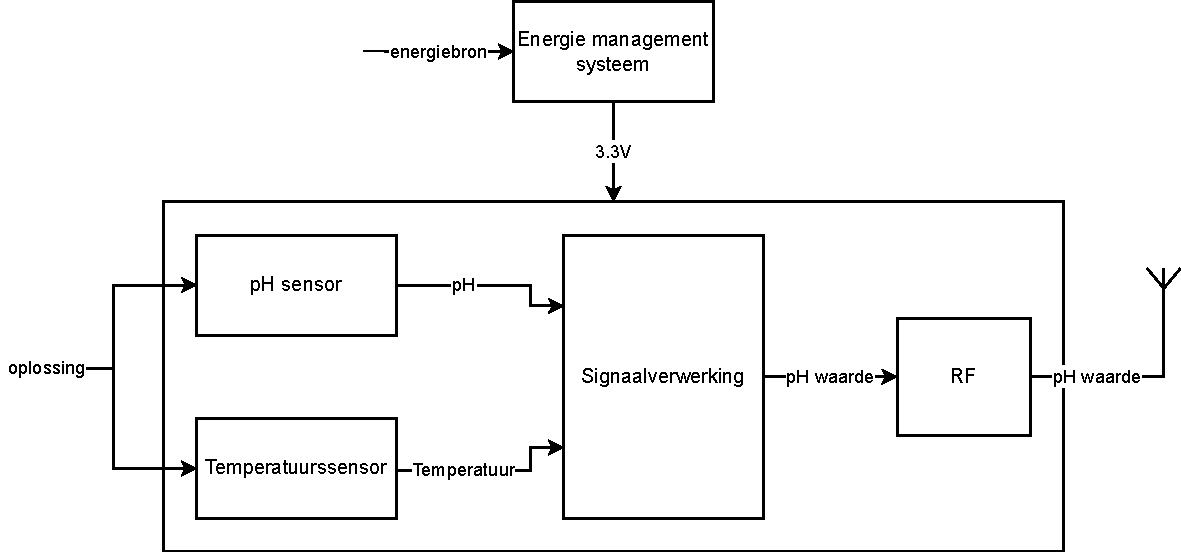
\includegraphics[width=\textwidth]{moduleDiagram.pdf}
    \end{figure}
    
\end{frame}



\subsection*{Eisen}
\begin{frame}
    \frametitle{Systeem eisen}

    \begin{table}[ht]
        \centering
        \begin{tabular}{|l|c c|l|}
            \hline
            Beschrijving                    & Min               & Max   & Eenheid           \\
            \hline 
            Afwijking                       &                   & 0.05  & pH                \\ 
            Bereik                          & 2                 & 10    & pH                \\
            Bandbreedte                     & 10                &       & Hz                \\
            $\mathrm{SNR}_{uit}$            & 36                &       & \qty{}{\decibel}  \\
            Rf afstand                      &                   & 10    & \qty{}{\meter}    \\
            Rf BER                          & $1\times10^{-5}$  &       &                   \\
            Levensduur                      & 48                &       & \qty{}{\hour}     \\
            Gemiddeld gebruikte vermogen    &                   & 10    & mW                \\
            Energy harvesting               & $>$ 0             &       & mW                \\
            \hline
        \end{tabular}
        \caption{Systeemspecificaties.}
        \label{tab:systemSpecs}
    \end{table}

\end{frame}
    
% \end{frame}
\subsection*{decompositie}
\begin{frame}
    \frametitle{Functionele decompositie}
%     \begin{figure}
%         \centering
%         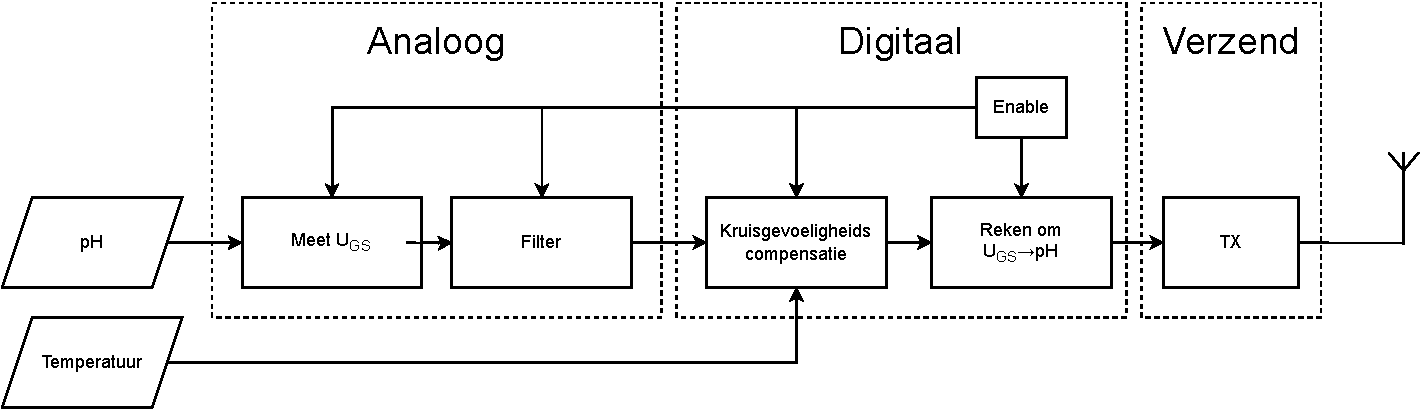
\includegraphics[width=\textwidth]{img/meetGedeelte.pdf}
%     \end{figure}
%     \begin{figure}
%         \centering
%         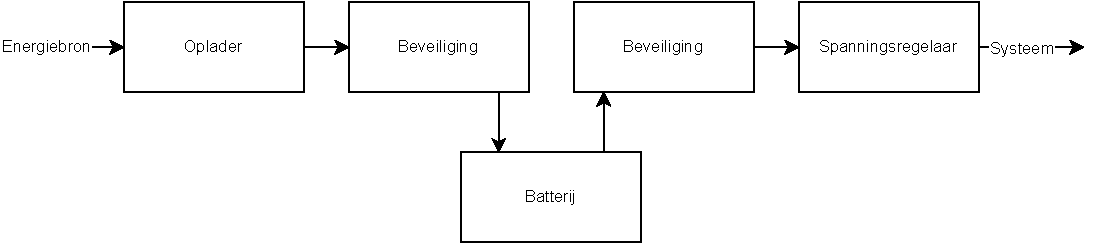
\includegraphics[width=\textwidth]{img/funcdDecompEnergy.pdf}
%     \end{figure}    
% \end{frame}
% \subsection*{Energie \& ruis}
% \begin{frame}
%     \frametitle{Energie \& ruisbudget verdelen}

%     SNR systeem uit = 34dB

%     \begin{table}
%         \centering
%         \begin{tabular}{l|l|l}
%             Func. blok          & Vermogen [mW] & NF [dB]   \\\hline
%             Reken $U_{GS}\rightarrow$pH & 0.6   & 3         \\
%             ADC                 & 1             & 3         \\
%             AA-filter           & 0.2           & 3         \\
%             Meet $U_{GS}$       & 0.2           &           \\\hline
%             Zenden              & 5             &           \\\hline
%             Oplader             & 0.5           &           \\
%             Beveiliging         & 0.5           &           \\
%             Spanningsregeling   & 1             &           \\ 
%         \end{tabular}
%     \end{table}

%     \pause

%     SNR Meet $U_{GS}$  $>43$dB

\end{frame}